We need to compute the largest eigenvalues of the filter \(W\).
The reason can be found by formulating the filter by its diagonalisation \(W = \sum_i^N \lambda_i \phi_i \phi_i^T\).
We know that the eigenvalues of \(W\) are non-negative.
When the \(i\)th eigenvalue \(\lambda_i\) is small and tends to 0, the eigenvector product will be negligible, and therefore the largest eigenvalues of the filter \(W\) are the most relevant.

For the approximation, we will actually need to compute the largest eigenvalues of the sampled pixels submatrix \(W_A\) to use the Nystr\"om extension.
Using a sample of the image, and thus of the matrix, to compute the largest eigenvalues works to approximate the complete filter because these eigenvalues are decaying rapidly as shows the figure below:
\begin{figure}[H]
  \centering
  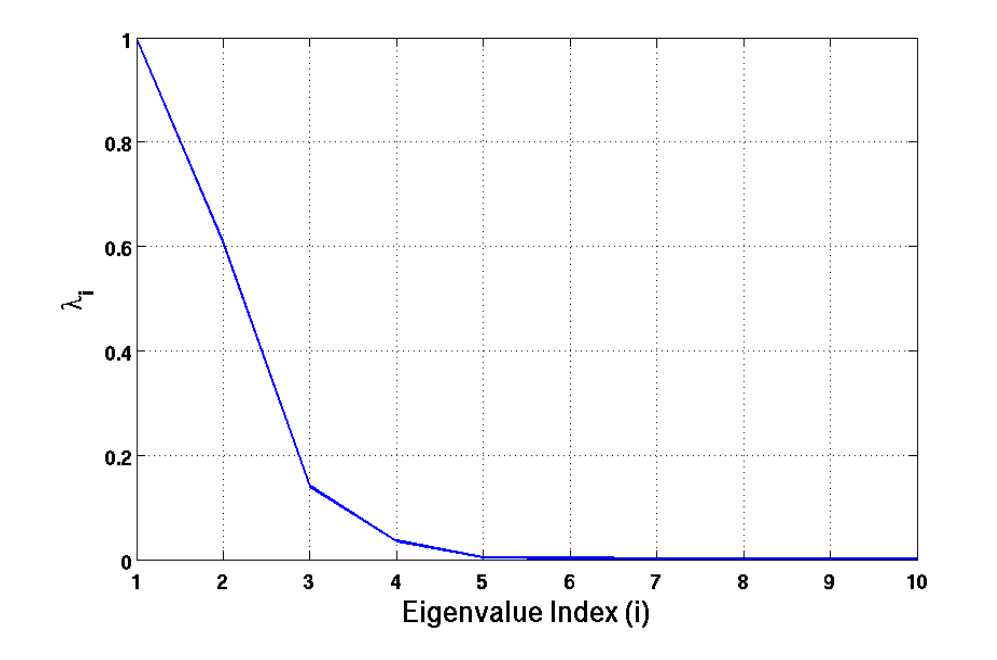
\includegraphics[width=0.9\textwidth]{img/decayingEigenvalues.png}
  \caption{Largest eigenvalues of an image filter, taken from \cite{siam_slides_2016}.}
\end{figure}
% TODO refaire soit meme

We know that the eigenvalues of submatrix\ \(W_A\) are between the extremum eigenvalues of the filter \(W\), which is known as the interlacing property of principal submatrices.
This can be proven with the Courant-Fischer theorem and the Rayleigh quotient.
We also know that computing the largest eigenvalues of the submatrix filter is equivalent to computing the smallest eigenvalues of the corresponding Laplacian operator.
This can easily be proven by the filter formula.
Let \(\lambda\) be an eigenvalue of \(W_A\) and \(x\) the associate eigenvector:
\begin{equation}
 \begin{split}
     W_A x = \lambda x & \Leftrightarrow (I - \Lapl_A)x = \lambda x \\
                     & \Leftrightarrow x - \Lapl_A x = \lambda x \\
                     & \Leftrightarrow \Lapl_A x = x - \lambda x \\
                     & \Leftrightarrow \Lapl_A x = (1 - \lambda) x
 \end{split}
\end{equation}

The goal of this observation is the way of computing the eigenvalues.
For the largest eigenvalues, the most famous algorithm is the power method.
For the smallest eigenvalues, the inverse power method is a usual choice.
Both methods converge faster when two successive eigenvalues are far from each other.
In broad strokes, the power method requires many cheap iterations, whereas the inverse iteration needs few expensive iterations.
In our case, the largest eigenvalues are close to each other; hence the inverse of these eigenvalues will be far from each other.
We will therefore prefer the inverse power method.

The algorithm will, in an iterative manner, compute the associated eigenvector of an eigenvalue.
This requires either to invert a matrix such as \(x_{k+1} = A^{-1} x_k\), or to solve the linear system \(A x_{k+1} = x_k\).
We will solve systems of linear equations to compute the first eigenvalues of the Laplacian in order to observe the behaviour of solvers on these dense matrices.

The main drawback of the Nystr\"om method for us, is that it approximates the leading eigenvalues but we compute the trailing ones of the Laplacian \(\Lapl\) \cite{belongie_spectral_2002}.
It is possible to obtain the eigendecomposition of the filter \(W\), even when \(W\) is indefinite, through a method proposed by \cite{fowlkes_spectral_2004}.
It consists of computing the inverse square root matrix \(W_A^{-1/2}\), which could be done either by the complete eigendecomposition or by using Cauchy's integral formula.
After this step, two more diagonalisation of matrices are required, demanding an important computation time.

Nevertheless, as stated in the objectives of the project, our main goal is not the image processing aspect, but the behaviour of linear solvers of these dense matrices using domain decomposition methods.
We will therefore stick to computing the smallest eigenvalues of the Laplacian operator \(\Lapl\) and avoid spending too much time on the end of the algorithm implementation.
